% @Author: AnthonyKenny98
% @Date:   2020-02-23 14:26:30
% @Last Modified by:   AnthonyKenny98
% @Last Modified time: 2020-04-05 08:02:21

\subsection{Hardware Acceleration}
    \Gls{hardware acceleration} refers to the strategy of using computer hardware specifically designed to execute a function more efficiently than can be achieved by software running on a general purpose \gls{CPU}.
    Specialized hardware designed to perform specific functions can yield significantly higher performance than software running on general purpose processors, and lower power consumption than \gls{GPU}s.

    \subsubsection*{Computer Implementation Hierarchy}
        To briefly frame the space in which this thesis operates, consider the typical computer implementation hierarchy, demonstrated in Figure \ref{fig:computerHierarchy}. \textbf{User level applications}, such as Google Chrome, Microsoft Word, and Apple's iTunes, sit at the top of the abstraction hierarchy. These applications are implemented in \textbf{High-Mid Level Languages}, such as C/C++, Python, Java, etc. These programming languages have their own hierarchy, but for the purpose of this thesis, it is sufficient to understand that these programming languages are then compiled into \textbf{Assembly Language}. Assembly language closely follows the execution of instructions on the \textbf{processor}, and is defined by an \textbf{\gls{ISA}}. An \gls{ISA} can be thought of as the contract between software programmers and processor engineers, agreeing what instructions the processor is able to implement. This assembly code is finally loaded into the processor's instruction memory and executed. 
        % @Author: AnthonyKenny98
% @Date:   2020-02-29 23:52:30
% @Last Modified by:   AnthonyKenny98
% @Last Modified time: 2020-04-10 12:37:43
\begin{figure}[H]
\begin{center}
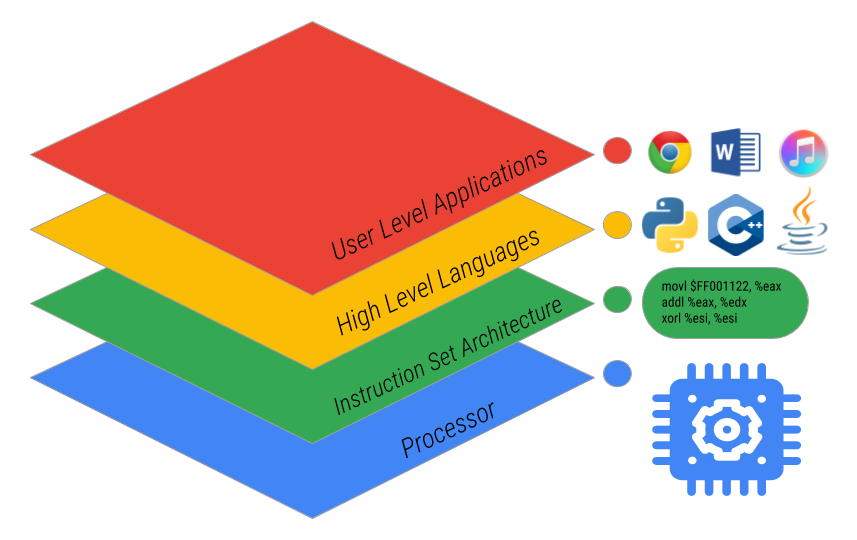
\includegraphics[width=\linewidth]{chapters/chapter1/img/computerHierarchy.png}
\mycaption{Simple Visualization of Computer Implementation Hierarchy}{}
\label{fig:computerHierarchy}
\end{center}
\end{figure}
        As will be outlined in Section \ref{section:projectOverview}, this thesis operates extensively on the lower two levels of this hierarchy, extending an existing \gls{ISA} and building hardware at the processor level that supports these extensions.

    \subsubsection*{Acceleration of Motion Planning}
        Accelerating motion planning with hardware is a fairly well studied problem. \\
        \textit{A Motion Planning Processor on Reconfigurable Hardware} \cite{Atay2006} studied the performance benefits of using \gls{FPGA}-based motion planning hardware as either a motion planning processor, co-processor, or collision detection chip. It targeted the feasibility checks of motion planning (largely collision detection) and found their solution could build a roadmap using the \gls{PRM} algorithm up to 25 times faster than a Pentium-4 3Ghz CPU could. \\
        In \textit{A Programmable Architecture for Robot Motion Planning Acceleration} \cite{Murray}, Murray et al. built on the work of the aformentioned paper, to accelerate several aspects of motion planning in an efficent manner. \\
        \textit{FPGA based Combinatorial Architecture for Parallelizing RRT} \cite{Malik2015} studies the possibility of building architecture to allow multiple \gls{RRT}s to work simultaneously to uniformly explore a map. Taking advantage of hardware parallelism allows systems such as this to compute more information per clock cycle. \\
        Finally, in the paper \textit{Robot Motion Planning on a Chip} \cite{Murrayb}, Murray et al. describe a method for contructing robot-specific hardware for motion planning, based on the method of constructing collision detection circuits for \gls{PRM} that are completely parallelised, such that edge collision computation performance is independent of the number of edges in the graph. With this method, they could compute motion plans for a 6-degree-of-freedom robot more than 3 orders of magnitude faster than previous methods.

    \subsection{RISC-V}
    \subsubsection{Extending RISC-V}
    RISC-V is designed cleverly in a modular way, with a set of base instruction sets and a set of standard extensions. As a result, processors can be designed to only implement the instruction groups it requires, saving time, space and power on instructions that won't be used. In addition, another goal of RISC-V is to provide a basis for more specialized instruction-set extensions or more customized accelerators. This is described in the most recent \textit{RISC-V Instruction Set Manual} \cite{Waterman2019}. This is a powerful feature, as it does not break any software compatability, but allows for designers to easily follow the steps outlined in Figure \ref{fig:extendingRISCV}. From a \gls{hardware acceleration} point of view, this is particularly useful as it allows the designer to directly invoke whatever functional unit or accelerator they implement from assembly code.
    % @Author: AnthonyKenny98
% @Date:   2020-03-01 10:28:34
% @Last Modified by:   AnthonyKenny98
% @Last Modified time: 2020-03-01 10:32:45
\begin{figure}[H]
\begin{center}
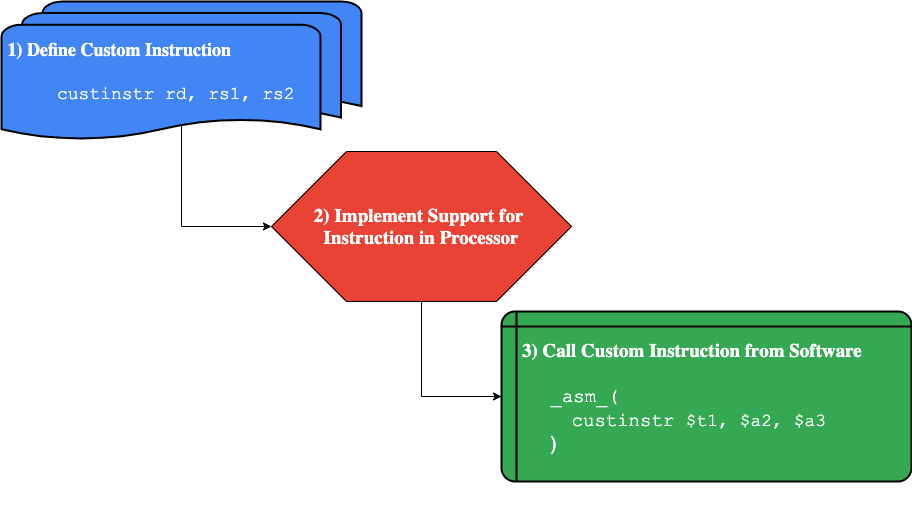
\includegraphics[width=0.9\linewidth]{chapters/chapter1/img/extendingRISCV.png}
\caption{Typical Process of Adding Non-Standard Extension to RISC-V ISA}
\label{fig:extendingRISCV}
\end{center}
\end{figure}

    \subsubsection{Accelerating RISC-V Processors}
    Having only been released in 2011, RISC-V is still a relatively unexplored opportunity for non-education applications. However, it shows promise in the commercial space, with Alibaba recently developing the Xuantie, a 16-core, 2.5GHz processor, currently the fastest RISC-V processor. Recently there has been promising research into accelerating computationally complex applications, particularly in edge-computing, with RISC-V architecture. \\
    \textit{Towards Deep Learning using TensorFlow Lite on RISC-V}, a paper co-written by the faculty advisor of this thesis, V.J. Reddi, presented the software infrastructure for optimizing the execution of neural network calculations by extending the RISC-V ISA and adding processor support for such extensions. A small number of instruction extensions achieved coverage over a wide variety of speech and vision application deep neural networks. Reddi et al. were able to achieve an 8 times speedup over a baseline implementation when using the extended instruction set.
    \textit{GAP-8: A RISC-V SoC for AI at the Edge of the IoT} proposed a programmable RISC-V computing engine with 8-core and convolutional neural network accelerator for power efficient, battery operated, IoT edge-device computing with order-of-magnitude performance improvements with greater energy efficiency. \\

